% REMEMBER: Write the thesis from the view of the reader. How would I like to READ the thesis?
% WHY -> WHAT -> HOW structure

\chapter{Future Work}

% What does this work already present?
Although Whisker is pretty usable in its current form,
there are still many opportunities for improvement:
\parspace

\textbf{Automated input.}
While Whisker's automated input algorithm works quite well, it is still very simple.
One could use more elaborate static analysis to find better fitting inputs.
For example, the optimal duration of a key press and its probability may be determined through static analysis.
At the same time, the algorithm may construct correct answers to \texttt{ask} blocks at run time.
Figure~\ref{fig:generated_ask_answer} shows ask-answer configuration from one of Code Club's sample solutions,
for which answers may be generated.

\begin{figure}[htpb]
    \centering
    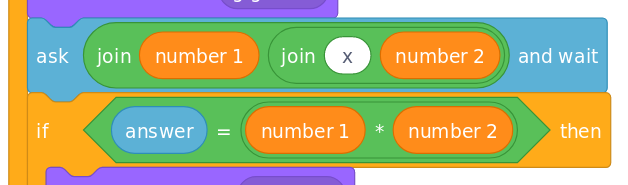
\includegraphics[width=0.4\textwidth]{scratch-ask-answer}
    \caption{Ask-answer configuration with a generated question and answer}
    \label{fig:generated_ask_answer}
\end{figure}

\textbf{Simplify tests with helper methods.}
Tests with Whisker can quickly become quite long and complex.
Therefore, helper methods to simplify testing should be provided.
For example, checking temporal relationships between two events,
e.g. "one second after some sprite touches a border, some variable must be increased",
currently requires a large amount of code.
In the future, methods to handle procedures like this could be provided,
which could simplify testing greatly.
\parspace

\textbf{Support for audio and Scratch extensions.}
Whisker could be extended to support sounds and Scratch extensions.
Scratch has a small number of extensions, which add blocks with various functionality.
For example, the "Pen" extension allows to freely draw on the stage by controlling a pen through the program,
and the "Video Sensing" extensions allows to detect movement with a web cam.
Adding support for audio as well as extensions in the future would allow Whisker to be used on a wider range of Scratch projects.
\parspace

\textbf{User interface.}
Another thing, that can be expanded upon, is Whisker's user interface.
Currently Whisker only has a web GUI, which is accessed through a web browser.
This interface can be used to test projects in batch, but it still requires a user to select he programs and tests manually,
and to manually save the test report once the test execution finished.
In the future, a standalone Electron~\cite{electron} application could save these problems.
It would also make it possible to run tests in parallel on a cluster.
